\chapter{The Transmission Puzzle} \label{chapter-tramsmission}%{Distribution and Growth} \label{chapter-distribution}
% \chapter{Productivity Spillovers} \label{chapter-productivity-spillovers}

\epigraph{Alternative micro-foundations cannot be regarded as interchangeable contents for the black box \dots %The micro-foundations of urban agglomeration economies interact with other building blocks of urban models in ways that we cannot recognise unless they are explicitly stated. For instance, the composition of cities typically emerges as a consequence of the scope of different sources of agglomeration economies and their interaction with other aspects of individual behaviour. Third, 
different micro-foundations have different welfare and policy implications. %If we begin building an urban model by postulating an aggregate production function with increasing returns, we can only take this function as given. If instead we derive this aggregate production function from first principles, we may see that its efficiency can be improved upon. The means for achieving such an improvement will depend on the specifics of individual behaviour and technology. Thus, while different assumptions regarding individual behaviour and technology may support similar aggregate outcomes, the normative implications of alternative micro-foundations can differ substantially.
}{Duranton and Puga \cite{durantonMicroFoundationsUrbanAgglomeration2004}}

\epigraph{A large body of literature documents the existence of agglomeration economies in developed economies ... The main conclusion of this literature is the finding of scale economies of 3--8 percent (that is, a 10 percent increase in the size of an activity in a city raises productivity in this activity by 0.3--0.8 percent).}{Gilles Duranton \cite{durantonAreCitiesEngines2009}} % (see Rosenthal and Strange 2004 for a review).




In Chapter~\ref{chapter-growth} we showed that two lines of research, growth theory and work on urban scaling, have settled on one of the most robust ``stylized facts'' in economics: wealth scales superlinearly with density. Substantial empirical research has shown that the general relationship\footnote{We use $\beta$ here because it is the most common form in the literature on urban agglomeration, although elsewhere we use $\gamma$, $\alpha$ and $\beta$ for the coefficients on capital and labour respectively as is most common in the economics literature.} between population and output at the urban %is well approximated by 
follows Equation~\ref{eq-agglom-eqn2}: \cite{loboUrbanScalingProduction2013}.

\begin{equation}\label{eq-agglom-eqn2}
    Y=AN^\beta,\qquad \beta>1. 
\end{equation}

Although research consistently finds strong agglomeration effects, there is a great deal of variation in the estimates. McCoskey and Kao \cite{mccoskeyPanelDataInvestigation} show that the impact of urbanization on growth varies greatly across countries in different countries, however. The World Bank (2016), for example, reported that every 1\% growth in urban population correlates with an increase in GDP per capita by 13\%, 10\%, and 7\% in India, China, and Thailand, respectively. Indonesia realizes only 4\% GDP growth for every 1\% increase \cite{haryantotriRelationshipUrbanizationEducation2021}. Interestingly the residuals or unexplained components for smaller cities are much larger than they are for large cities, as Figure~\ref{fig-residuals-lobo} from Lobo et all \cite{loboUrbanScalingProduction2013} illustrates.\footnote{The observation suggests that clues about the mechanisms may be found by examining smaller and mid-sized cities and that potential policy impacts may be greater for these cities.} the literature has not yet settled on an explanation of the variation.  \cite{loboUrbanScalingProduction2013, pugaMagnitudeCausesAgglomeration2010} 



\begin{figure}[h!tb]
\centering
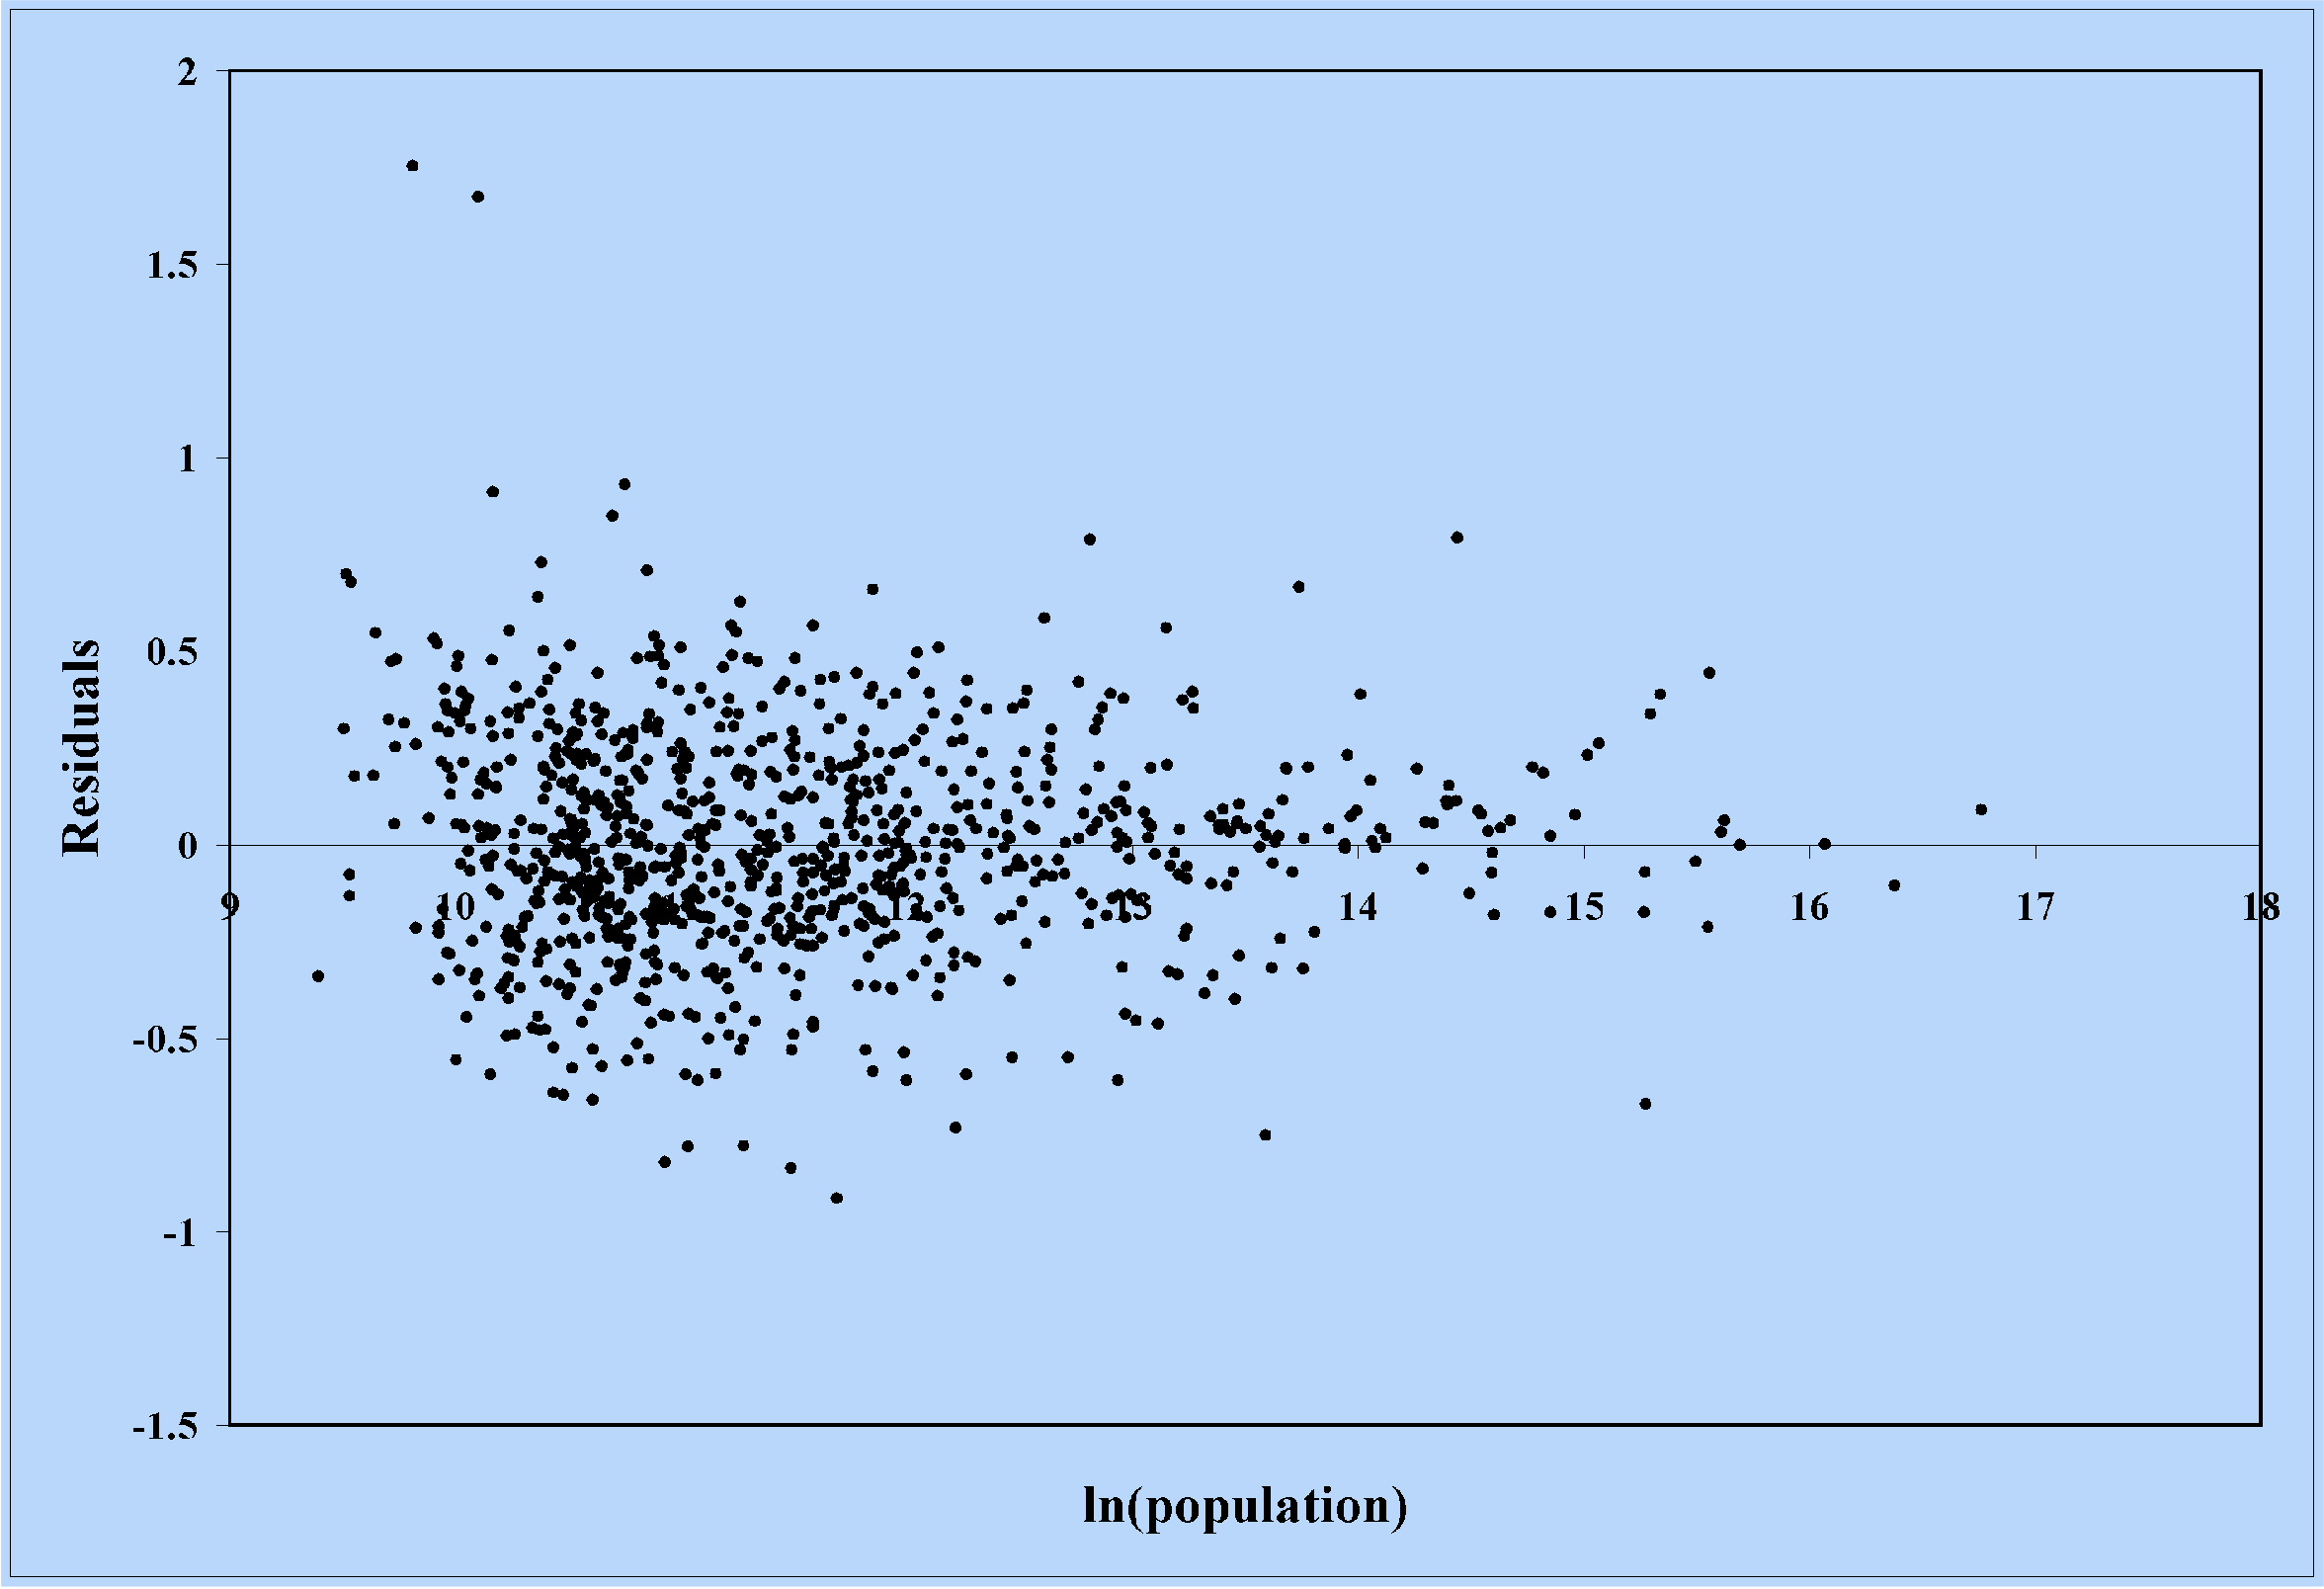
\includegraphics[scale=0.30]{fig/residuals-lobo.png}
\caption{Residuals from regressing ln(total wages) on ln(population) using data for all 943 urban areas of the United States showing larger unexplained components for smaller cities. \cite{loboUrbanScalingProduction2013}.}
\label{fig-residuals-lobo}
\end{figure}

The variation in estimates suggests there may be multiple and variable channels affecting the magnitude of agglomeration effects.  This raises the possibility that there are several channels for public policy to enhance the positive effects of agglomeration.  If the agglomeration parameters $A$ and  $\beta$ can be affected positively by policy choices, or perhaps negatively by trends such as financialization,  governments may be able to significantly increase social wealth and well-being. In addition, the variation suggests that that financialization may have an impact through multiple channels.  Understanding the mechanisms has  considerable policy importance.

% the channels through which the effect works are not clearly understood. 

% In particular, how the changes induced by financialization of the housing market might affect the fundamental productivity of the city has not been explored.



{\color{red} In the next section we discuss potential linkages  with reference to the two dominant theoretical frameworks for understanding agglomeration effects, %. Second, it introduces the micro-foundations, the mechanisms by which agglomeration happens, drawing on the literature, and discussing how financialization might affect those mechanisms. Finally, in section~\ref{section-impact-channel-summary}, we summarize the primary linkages as they might appear in our model.
} 

\section{Impact channels}
Identifying channels through which the policies or trends might affect productivity is important for this work because by introducing the linkages into our model explicitly, we can test the model's sensitivity to a range of policy interventions and lay the foundation for empirical work. %Identifying these linkages is important but it is complicated on at least two levels. First, the micro-level mechanisms driving productivity gains in the production sector, themselves are not well understood.  Second, the linkages between urban productivity and financialization have not been established.  
Figure~\ref{fig-impact-channels} illustrates some of the channels through which the financialization of housing might impact city productivity. 
In the figure, the production sector is on the right, the processes occurring within the city are central, and the speculative intervention in the housing market is to the left.  \footnote{The figure only shows some of the links and feedbacks we discuss. It is not our intent in this chapter to provide  a comprehensive discussion of any of the linkages we examine. Each of the linkages shown or mentioned warrants extensive research, and for most even a brief literature search will reveal many related papers.} 

% {\newpage\thispagestyle{empty}
% \vspace{-1.5cm}
\begin{figure}[h!tb]\label{fig-impact-channels}
%\vspace{-1cm}
\begin{adjustwidth}{-0.24\textwidth}{-0.24\textwidth}
\centering
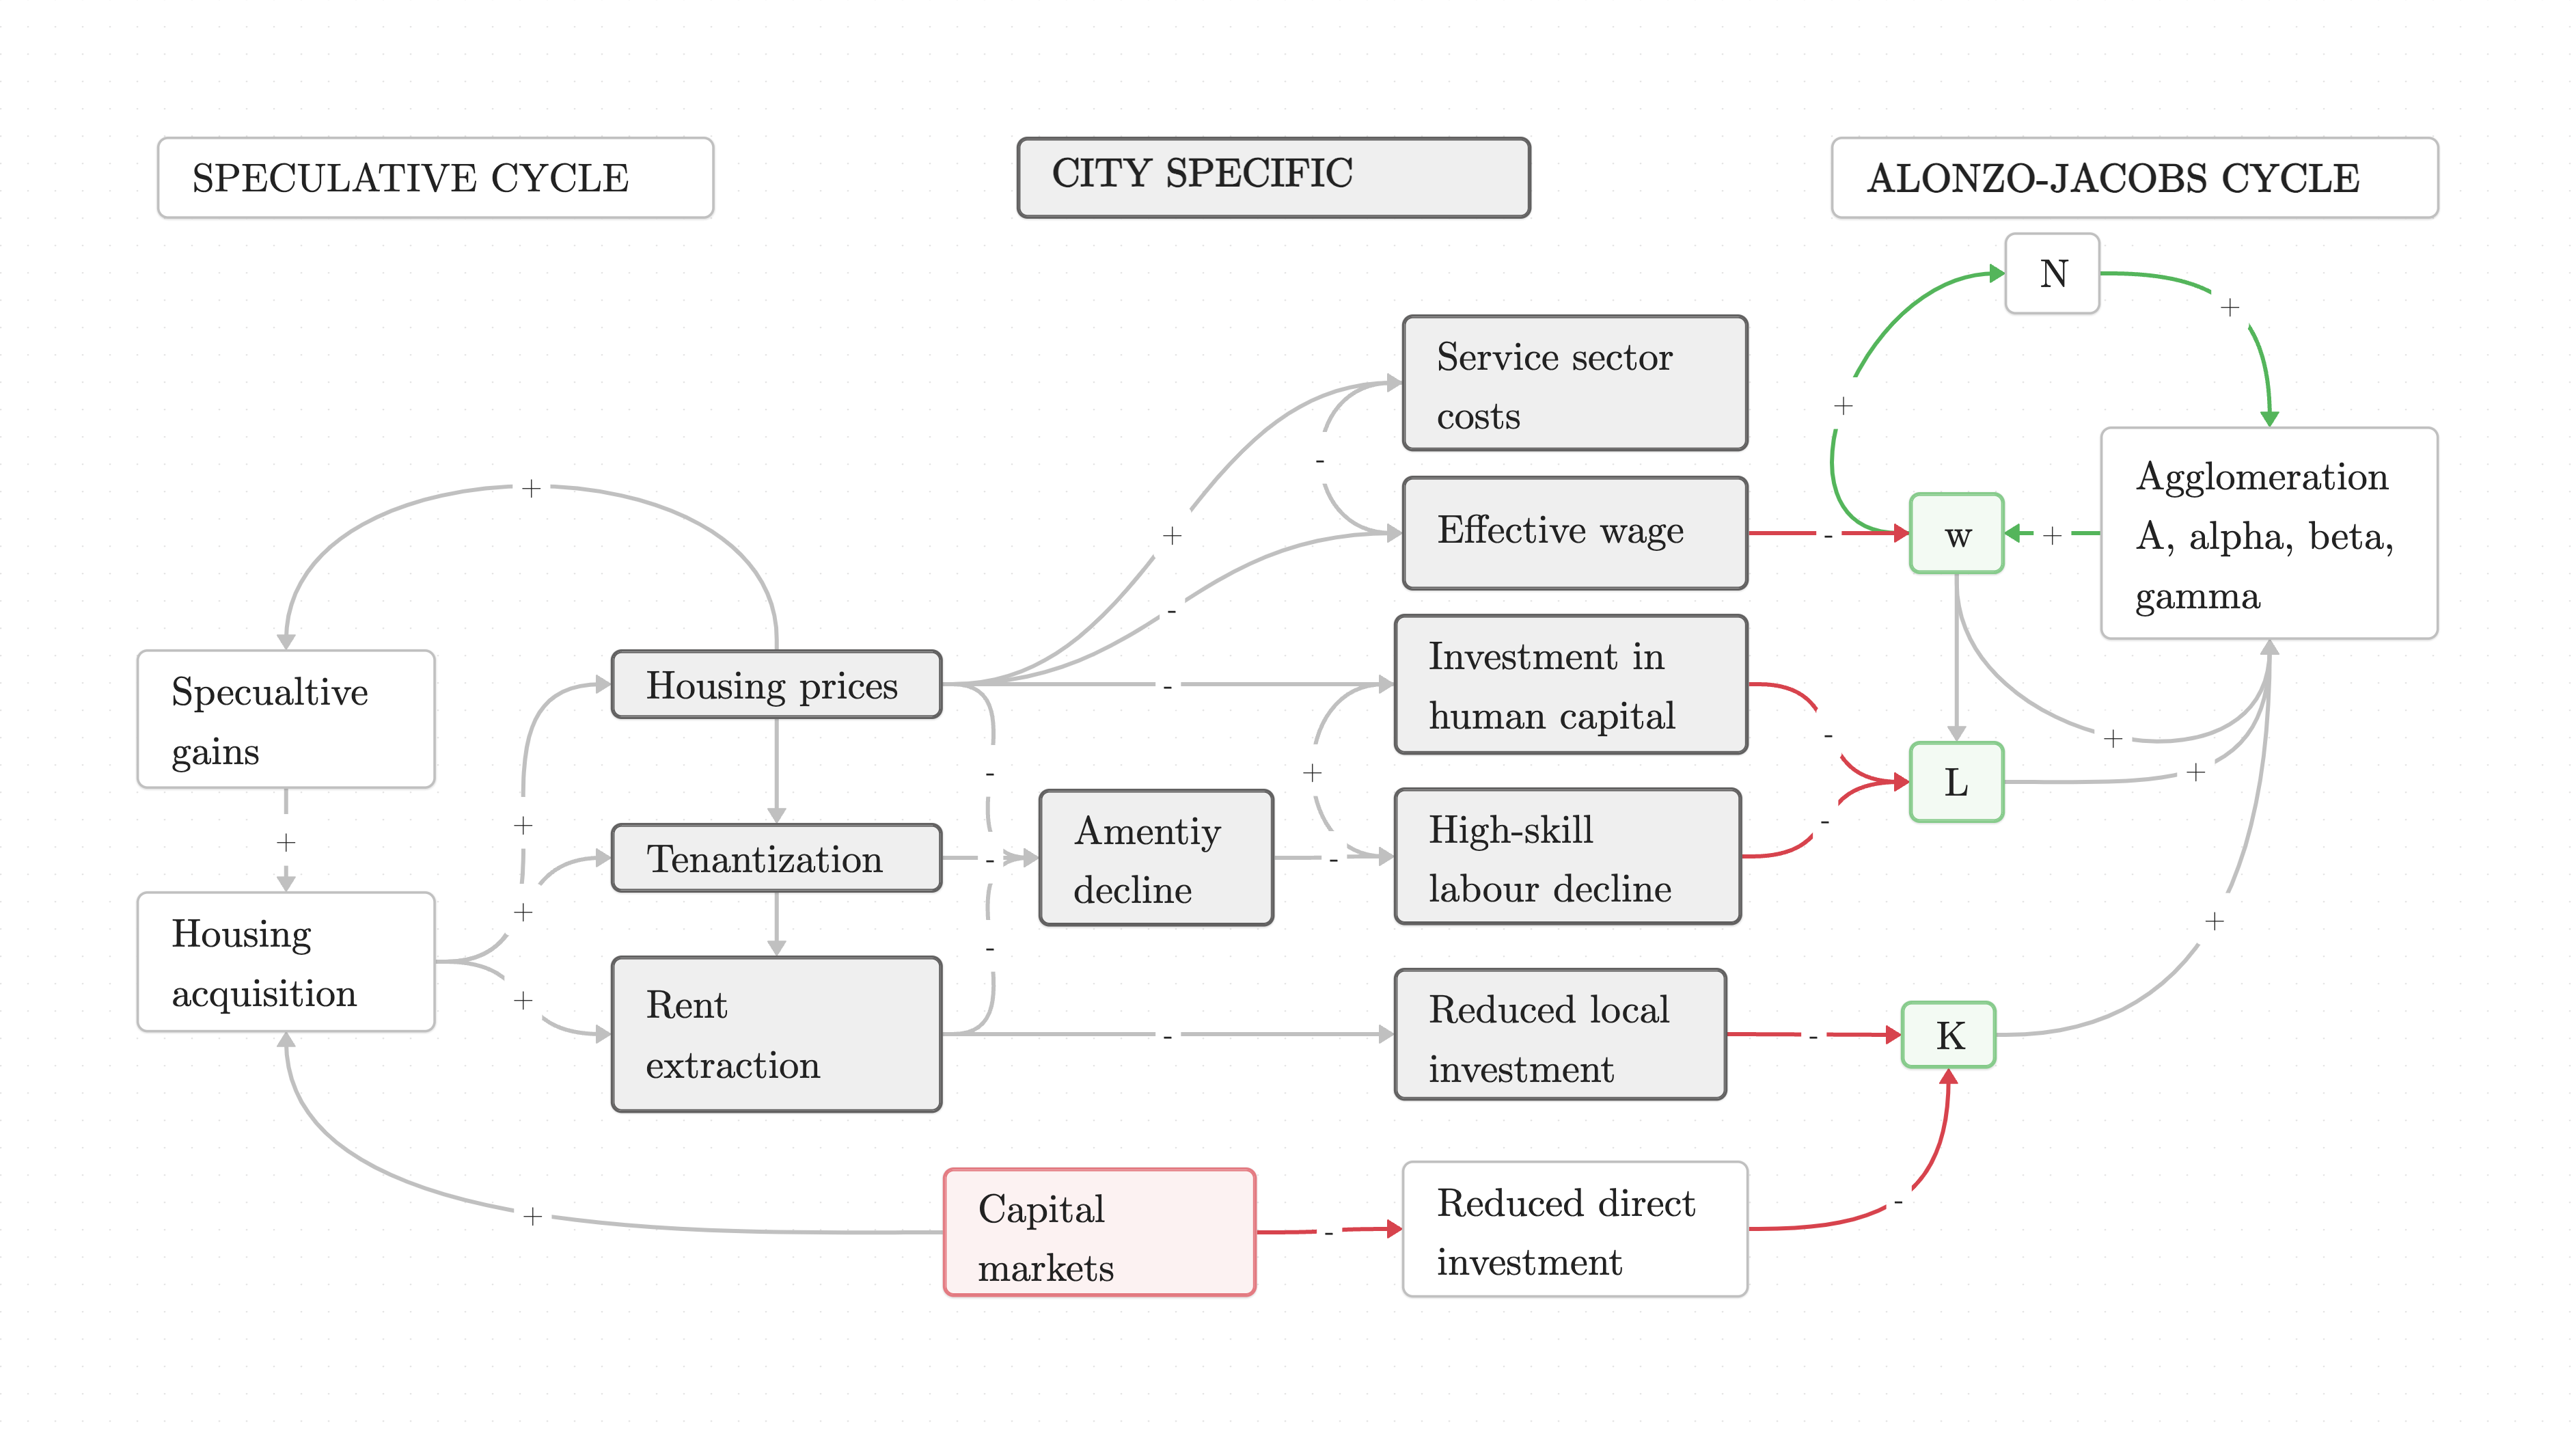
\includegraphics[scale=.15 ]{fig/impact-channels.png}%angle=90
\end{adjustwidth}
\caption{Impact channels relating financialization and urban productivity.}
\end{figure}
%}


In the upper right, we show the \gls{Alonzo-Jacobs cycle}, described in Chapter~/ref{chapter-model}. In it, the strength of the agglomeration effect determines productivity, which drives wages, which determines population which feeds back to agglomeration. In our model, anything that affects productivity must affect this cycle directly or indirectly.  We show the effect of interventions or financialization on productivity primarily through their effect on wages, labour supply and capital supply. %making it indistinguishable from the Jacobs model at the urban level. 

\subsection{Reduced capital stock}
We focus on the impacts of financialization as they work through the urban system rather than on effects that operate directly through real investment. Before we do, it is important to note that fiancialization has both direct and indirect effects. Financial markets are global and allocate capital to the most profitable sector.  
Marxist theorists \cite{lefebvreRevolutionUrbaine1970, harveyClassmonopolyRentFinance1974, harveyUrbanProcessCapitalism1978, christophersRevisitingUrbanizationCapital2011} have argued that finacialization diverts capital investment from productive investment to financial enterprises. 

This direct effect is illustrated at the bottom of Figure~\ref{fig-impact-channels}, where capital markets can divert capital from the productive activities on the right to speculative activities on the left. Switching happens in response to the relative rates of return on the two sides.  We allow the rate of return on housing to rise in response to city growth, attracting speculative investment. We can also simulate a falling rate of return on productive investment by reducing the cost of capital to investors or by inhibiting the rate of growth of capital on the production side in response to rising investment in housing purchases. % adjK



\subsection{Local investment}

Financialization may reduce the amount of local capital available, raising the cost of capital in the city. 
There are at least two mechanisms by which local investment capital may be affected. First, if increased tenantization and rent extraction reduce household wealth, we would expect household investment to decline. The decline would probably be correlated with a decline in direct investment, amplifying its effect. Furthermore, this channel would act very slowly and persist after an initial round of speculative activity. 

Second, because private production is complemented by public infrastructure, it is possible that the tenantization for the city would lead to declining municipal investment in public infrastructure. It is known, however, that municipalities generally spend less on tenants and collect more revenue per capita from rental as opposed to owner-occupied housing, so tenatization might lead to rising pressure for infrastructure expenditure.  We can capture these effects by linking the owner-occupier ratio to capital stock. A more detailed approach would explicitly allocate some of the municipal taxes to increasing the agglomeration parameters. 




\subsection{High-skill labour decline}

 Speculation and rising housing prices that result in tenantization will make a city less attractive to highly skilled labour, making it more difficult to attract or hold people with the specific adaptive skills Glaeser and Saiz \cite{glaeserRiseSkilledCity2003} identified. Slowing in-migration or increasing out-migration of the more skilled members of the labour force  will \textit{ceteris paribus} reduce the effective supply of labour. 
Liu et al \cite{liuImpactUrbanHousing2023}, for example, found for China that and increase in urban housing prices has a crowding-out effect on labour mobility.  Duffy et  \cite{duffyRisingHousePrices2005} found that for Ireland that rising house prices, by discouraging potential migrants, could significantly reduce the growth potential of the economy, shifting the balance of labour market growth from employment to wages, with a consequent deterioration in competitiveness. %Anecdotal evidence comes from comes form the frequent news stories about which cities are most livable: low housing prices are almost always an important element in the measures used. (we omit the link form  housing prices to high-skill labour. 

Althobaiti et al \cite{althobaitiHousingPricesSkills2021}  show that with gentrification, high-level cognitive skills are getting closer to the city center in response to the increase of median housing prices while low-level physical skills got further away.  Gentrification can be seen as trend opposing tenantization. The effects of tenantization, neighborhood decline and disinvestment, which Cornelissen and Jang-Trettien \cite{cornelissenHousingContextNeighborhood2023} point  are more common than gentrification in low-income neighborhoods, are likely to be opposite of the effects of  gentrification.

The reduction might be offset by importing human capital, though immigration or rising wages for talent in the city. Florida\cite{floridaCompetingAgeTalent2005, floridaCreativeClassEconomic2014} has suggested that urban growth is strongly linked to the ability to attract talent. 

We can introduce this channel by making  the labour elasticity of output in the Cobb-Douglas function, $\beta$, depend on the home-ownership ratio.  


\subsection{Reduced investment in human capital}

There is a vast literature on investment in human capital. 
Growth theory associates increasing returns to scale in the industrial sector or at the national level with increasing effective human capital, which grows faster than the labour supply as a result of increased education, as we described in Chapter~\ref{chapter-growth} section~\ref{section-growth}. 
Growth theory suggests that the growth of human capital is  a major driver of productivity.  At the national level, Solaki \cite{solakiRelationshipEducationGDP2013} demonstrates a causal relationship between education and growth, and that tertiary Education should be considered as an exogenous variable.  Empirical results for Bangladesh \cite{islam2007relationship}show evidence of bidirectional causality between education and growth.  Among others, B\"uchler et al have recently confirmed the important of human capital growth for urban growth.

There are at least two mechanisms by which investment in human capital may be affected indirectly by financialization. The most direct is by reducing household incomes The effect may be different for different parts of the population. Increasing housing prices increases the wealth of owner-occupiers. this wealth effect may result in increased spending on education for offspring. Increased housing costs for tenants, on the other hand,  may result in reduced human capital investment.\footnote{Glaeser and Saiz found evidence for skill upgrading in declining cities, which suggested to them efficient investment in less skilled workers is a key adaptive/growth mechanism. If powerful enough this effect might offset some of the negative impacts of financialization we has suggested.}  

Less directly, we suspect financialization will increase the cost of living through, for example, increasing labour costs in the service sector. This results in a reduction of the effective wage, also reducing income available for human capital investments. Rent capture leading to reduced local capital of reinvestment in human capital might reduce the adaptive capacity of a city's population.

We can simulate some human capital effects simply by making a link from the home-ownership ration to the productivity parameters.



\subsection{The effective wage}

Purchasing power depends on the money wage and on the price level. inflation coming from the right side of the figure will reduce the effective urban wage, which Lobo et al. find is one of the determinants of growth. 

 Rising housing prices and rising rental prices reduce the purchasing power of city dwellers in more than one way. In addition to the direct effect, the rising housing costs make other goods and services more expensive. The wage of the Barista must go up, so the cost of a coffee has to rise. Bookstores may close, reducing the neighbourhood amenity level. 
 
 Local amenities may also be affected. Urban amenities  are part of the incentive for choosing city life for many, and any decline in amenity will have the same qualitative effect as a decrease in the wage. The size of the effect will vary because people's tastes differ. 


 General financialization may also reduce the bargaining power of labor, as Tomaskovic-Devey and Lin argue \cite{tomaskovic-deveyFinancializationCausesInequality2013}, reducing wages.\footnote{Tomaskovic-Devey and Lin point to a shift in behaviour of non-finance firms away from production and non-financial services and toward financial investments and services. This shift, they argue,  has led to lower employment, income transfers to executives and capital owners, and increased inequality among workers \cite{tomaskovic-deveyFinancializationCausesInequality2013}}
%In the second part of the chapter we implement several of the mechanisms and share results. 

% VERY INTERESTING \cite{buchlerImpactHumanCapital2024} in areas with elastic housing supply, the positive demand shock leads to the construction of more housing, a larger labour force, and, thus, moderate wage growth. In contrast, in areas of low housing supply, the positive demand shock has a limited impact on new housing construction and the urban population. Human capital gets capitalised into higher home prices, hindering urban growth.

\subsection{The amenity channel}
Rent capture might influence the concentration of educated personnel by reducing the diversity and amenity of cities, making urban living less attractive, reducing labour supply, or raising its cost.


\subsection{impact on the service sector}
Rising housing costs at the centre of a city would tend to push low-wage workers to the edges, increasing their transportation costs, putting further upward pressure on wages, and increasing the costs of all amenity services that rely on lower-cost workers.



\section{Theoretical frameworks} % Theoris of agglomeration}
{\color{green}The literature has produced two core theories about the source of agglomeration economies and identified many channels that are likely to affect the overall productivity of individual cities. The theories that have dominated the discussion of how agglomeration increases productivity are:}

%, Puga \cite{pugaMagnitudeCausesAgglomeration2010} did a review in 2010 and concluded that the literature had been so far unsuccessful at distinguishing between the possible sources of agglomeration effects. %despite broad agreement on the magnitudes.     
% can be expressed as Y (\lambda N)~Z(\lambda,N)Y (N). When the scale factor Z depends only on \lambda, i.e. Z(\lambda,N)~Z(\lambda), equation (2) can be solved uniquely to give the scale-invariant result of equation (1), with Z(l\lambda)~\lambda^\beta.
% The empirical results from the scale literature  make it clear that cities do  
%Empirical estimates of $\beta$ also vary. \cite{rosenthalEvidenceNatureSources2004, bettencourtIntroductionUrbanScience2021, loboUrbanScalingProduction2013}. 
 %In this section,  we try to identify the specific impact channels by which that financialization might affect one or more of these processes. 
% \section{Linkages and spillovers}

\begin{enumerate}
\item The Marshall-Arrow-Romer (MAR) growth theory emphasizes effects among firms in an industry.  Marshall (1890) described how the concentration of an industry in a city helps knowledge spillovers between firms and, therefore, the growth of that industry and of that city.\footnote{Glaeser et al. \cite{glaeserGrowthCities1991} tested a model of employment growth (not productivity growth) in an industry in a city as a function of the specialization of that industry in that city, local competition in the city-industry, and city diversity. None of their results support the importance of within-industry knowledge spillovers for growth. %If such spillovers. %This may be usefull for us because it rules out a  difficult channel to examine.
} More recently Porter (1990) began with a theory of industrial clusters at the national level and moved to the view that competition and cooperation within local concentrations of industry drives innovation and growth. The model. A variant of the  MAR model, the Porter model also ascribes agglomeration effects and technological spillovers to industry structure and none to urban structure or population per se.  

\item  In contrast, the \gls{Jacobs model} %, unlike the MAR and Porter models, 
suggests that important knowledge transfers come from outside the core industry through cross-fertilization among a variety of industries and even occur between individuals.

This is an essentially urban model without an explicit role for industrial structure or national levels of human capital.  The growth theorists, MAR AND PORTER focused primarily on industrial density and diversity, and the Jacobs theory focuses on population density as well as diversity. Neither approach considered financial variables.
\end{enumerate}




 Glaeser, Kallal, Sheinkman and Shleifer attempt to compare these theories empirically \cite{glaeserGrowthCities1991}. They used data from 170 of the largest US cities to study which industries grew fastest, in which cities, and why, between 1956 and 1987. %They found that industries grow slower in cities in which they are more heavily over-represented and faster where the firms in the industry are smaller than the national average and when the city is less specialized. 
This evidence was ``negative on MAR, mixed on Porter, and consistent with Jacobs.'' Scherer \cite{schererInterindustryTechnologyFlows1982} presented systematic evidence indicating that around 70 percent of inventions in a given industry are used outside that industry, generally supporting the Jacobs hypothesis that knowledge spills over across industries because cities bring together people from different walks of life and foster the transmission of ideas. Grilliches and Lichtenberg also examined R\&D spillovers but concluded the evidence about which channels are effective remains tenuous \cite{grilichesInterindustryTechnologyFlows1984}. Beaudry and Schiffauerova proposed that levels of aggregation together with the choice of performance measures are the main causes of the lack of resolution in the debate \cite{beaudryWhoRightMarshall2009}. The debate about which theory is the best description continues. 



% https://renx.ca/renters-often-pay-higher-municipal-taxes-than-homeowners




%.  REFERS to a figure that haas been removed
%The challenge to our to directly linking employment to the wage is that the firm will base its hiring decision on the red line, or at best the blue line, but it will not perceive or  respond to externalities incorporated in the green line.  The argument implies  that cities will be chronically inefficient, failing to grow as  much and as quickly as they should because private decision-makers fail to take into account the agglomeration externalities. 

% \section{Micro-foundations} % of agglomeration}
%To model the relationship between production and population explicitly in an agent-based model, we need a more granular model/representation/theory of the mechanism that links population and productivity. We need to understand the impact channels. 
% The broader thereretical framework only goes so far howerver. 

%These high-level theoretical relationships operate through specific mechanisms at a micro level. In this section, we introduce those mechanisms and speculate about the potential impact financialization might have on the productivity gains that come from agglomeration effects.

\section{Empirical results}

As we observed in Chapter~\ref{chapter-growth}, both growth theory and urban scaling rely on %general 
notions of `knowledge spillovers,' `network effects,' and variants of `specialization" to explain the phenomenon.  They do not agree on precisely how the effects of agglomeration are transmitted from demographic, spatial, or financial variables to overall city productivity and what modulates those effects, however. Duranton and Puga % \cite{durantonMicroFoundationsUrbanAgglomeration2004} focus on more directly on these channels: ``[u]rban agglomeration economies are commonly classified into those arising from labour market interactions, from linkages between intermediate- and final-goods suppliers, and from knowledge spill-overs.'' 
provide a classification for the mechanisms driving the link \cite{durantonMicroFoundationsUrbanAgglomeration2004}.  They argue that``[u]rban agglomeration economies are commonly classified into those arising from labour market interactions, from linkages between intermediate- and final-goods suppliers, and from knowledge spill-overs,''\footnote{Duranton and Puga's classification loosely follows the three main examples provided by Marshall \cite{marshallPrinciplesEconomics1890} in his discussion of the sources of agglomeration economies.} and go on to offer an alternative based on three types of micro-foundations for agglomeration:
\begin{enumerate}
\item sharing,
\item matching, 
\item learning mechanisms.
\end{enumerate}
In addition to these micro-foundations, we consider effects of investment in innovation\footnote{Innovation might be classified as a type of learning. We focus on the investment in innovation and treat that as a kind of capital investment.} and social inequality.

{\color{red}

 
\subsection{Sharing}
MAYBE SOME LINK MISSING HERE. I FIND I STOP READING PART WAY THROUGH THIS SECTION.
For Duranton and Puga, sharing gains arise because a larger final-goods industry will support a larger pool of input suppliers who can offer the gains from their specialization. This is an application of one of Adam Smith's main insights. Rosenthal and Strange \cite{rosenthalEvidenceNatureSources2004} find the effect of sharing a common base of suppliers is weak relative to other motives for agglomeration, while  Overman and Puga \cite{overmanLaborPoolingSource2010} find strong support for input sharing as a motive for agglomeration at the sector level. We do not explicitly introduce sharing, but it is captured in our model as a scale effect that then increases productivity by increasing $\beta$ in Equation~\ref{eq-agglom-eqn2}. 

It is not obvious that financialization will significantly affect the scale of industry, or the number of suppliers, but financially-driven mergers and acquisitions frequently lead to reducing the workforce and cutting wages. Investment in innovation may be cut in pursuit of short-term increases in share price.  Rising inequality might also limit the diversity of consumption choices which functions indirectly as a component of the effective urban wage. 

WHERE SHOULD THIS GO? Henderson \cite{Henderson1972Sizes} suggested that urbanization increases final market demand and diversity of products. Glaeser et al. \cite{glaeserGrowthCities1991a} suggest that this effect does not drive growth. 
 
\subsection{Matching}
MATCHING IS.. 
Matching mechanisms create increasing returns by cutting search costs for producers and by increasing the quality of matches. As the workforce grows and the number of firms increases, the average worker can find an employer that is a better match for his or her skill set. This appears as an improvement in effective labour. Matching occurs in a developed labour market with a specific set of informational institutions. It would probably require quite large changes in the labour supply or churn to cause a noticeable difference in matching speed or success rates. It is unclear how financialization could affect the matching process.

Duranton and Puga demonstrate that specialization by workers can generate increasing returns. Indirect mechanisms through which financialization might affect productivity restrictions on employment or wages might limit the diversity of the labour pool, reducing the range of locally produced products or services.  We do not explicitly introduce workforce diversity, but it follows that any mechanism that reduces the diversity of the workforce could eventually reduce productivity. These channels are incorporated in Figure~\ref{fig-impact-channels}.
 
\subsection{Learning}
Similarly, a variety of learning-based mechanisms have been suggested, FOR EXAMPLE but none that might obviously be affected by financialization. TODO ADD A SENTENCE OR TWO MORE

Spillover effects from learning can be large. Irwin and Klenow  studied learning in chip production focusing  on the key issue of spillovers. They found learning rates of 10 to 27 per cent, averaging 20 per cent. They indicated that a good part of learning is internal, and that national spillovers were no greater than international spillovers. " \dots a firm learns three times as much from an additional unit of its own cumulative output as from another firm's cumulative output, regardless of the other firm's country of location. However, rest-of-world cumulative production is typically more than three times any given firm's cumulative production. This means that the absolute contribution of world cumulative production to each firm's experience outweighs the absolute contribution of its own cumulative production. In this sense, spillovers are substantial." (pp. 1217-1218).

At this stage, it is difficult to see how the industry-based mechanisms he considered might be directly affected by increasing financialization. 


\subsubsection{Human capital, education, and hysteresis}

At the urban level a study by Glaeser and Saiz \cite{glaeserRiseSkilledCity2003} for the US found that human capital predicted population and productivity growth at the city and metropolitan area level as surely as it predicts income growth at the country level. 

They specifically found that cities with more educated residents have grown more quickly than comparable cities with less human capital. They find that causation running from growth to education seems to be present only in a handful of declining metropolitan areas, and cannot account for much of the relevant effect. Their evidence supports the view that skills induce urban growth.


% BEHIND WHAT RESULT? The intuition behind this result is a pure price effect. For cities that specialize in the skilled, their primary form of labor has become more expensive and as a result they grow less.

WHAT ARE human capital externalities?
Moretti (2003) extends Rauch (1993) and identifies human capital externalities by using instrumental variables related to human capital but plausibly exogenous to wages.11 He finds that, after controlling for the private returns to education, a 1 percentage point increase in the share of the college educated in a metropolitan area raises average wages by 0.6%-1.2%.

%the coefficient on schooling in housing price growth regressions is extraordinarily robust statistically when we control for initial housing price.

Panel A in Table 5 certainly seems to make it clear that higher levels of education increase both the population of metropolitan areas and the price that this population is paying for the privilege of living in the area. In Panel B (Table 5), we examine housing pr

What is the precise channel through which such advantages operate? Is it because a larger labor market improves matching between employers and employees? Or is it because large concentrations of employment iron out idiosyncratic shocks and improve establishments' ability to adapt their employment to good and bad times? Or perhaps because larger markets allow workers to specialize in a narrower set of activities and improve their performance? And how important are these advantages relative to alternative sources of agglomeration economies not operating through the labor market? % To answer such questions we need good models that formalize the microeconomic foundations of urban agglomeration economies, as well as detailed empirical work able to identify and quantify the precise mechanisms at work. This is an area where there has also been much recent progress. However, as we shall discuss in detail below, there are substantive open questions that forthcoming research ought to address.

%One of the fundamental results in spatial economics is Starrett's \cite{starrettMarketAllocationsLocation1978} spatial impossibility theorem. This states that, once we abstract from the heterogeneity of the underlying space, and without indivisibilities or increasing returns, any competitive equilibrium in the presence of transport costs will feature only fully autarchic locations where every good will be produced at small scales (see Ottaviano and Thisse, 2004, for a detailed discussion). Thus, substantial localization or spatial concentration of economic activity may be seen as a sign of agglomeration economies \cite{pugaMagnitudeCausesAgglomeration2010}.


%%%%.   Wage Premium
%Glaeser and Mare ́ (2001) \dots controlling for observable skills, instrumenting for urban residence using parental background, and finally exploiting the panel dimension of the data to include individual worker fixed-effects, \dots find that, even after all these corrections, there is significant wage premium associated with living and working in dense cities, although smaller in magnitude than before taking unobserved ability into account \cite{pugaMagnitudeCausesAgglomeration2010}.



%mechanisms to explain the existence of urban agglomeration economies
%First, a larger market allows for a more efficient sharing of local infrastructure and facilities, a variety of intermediate input suppliers, or a pool of workers with similar skills. Second, a larger market also allows for a better matching between employers and employees, buyers and suppli- ers, or business partners. This better matching can take the form of improved chances of finding a suitable match, a higher quality of matches, or a combina- tion of both. Finally, a larger market can also facilitate learning, for instance by promoting the development and widespread adoption of new technologies and business practices \cite{durantonMicroFoundationsUrbanAgglomeration2004}.

% RECENTLY7 REMOVED
         
%Based on this kind of research, we should expect that cities with universities will grow more quickly and that financialization might have either positive or negative effects on the growth of local colleges and universities. 


\subsection{Effects through innovation}
INNOVATION IS .. MIGHT EXPECT IT TO HAVE THESE EFFECTS.. 
Lobos et al. examined the simultaneous effects of spillovers due to research and development by universities and by firms \cite{belderbosWhatSpilloversUniversities2022}.

\begin{quotation}
``the formation and efficiency of agglomeration arise from its character as public capital; households and firms in the same agglomeration share its benefits in common. In contrast, an economic network is private capital shared primarily by the network participants. Agglomerations also rely on public institutions, which aggregate individual decisions. In contrast, economic networks arise from a collective decision by group members, generating a private institution. Networks are clubs in which exclusion is possible and price discrimination is the norm. Agglomerations cannot exclude economic actors from receiving benefits nor can they price these benefits efficiently.''
\end{quotation}
They point out, drawing on Dixit and Stiglitz \cite{AvinashK.Dixit1977MCaO},  Fujita \cite{fujitaMonopolisticCompetitionModel1988}, Stiglitz and Venables and \cite{fujitaSpatialEconomyCities1999} that economies of scale  can arise with the diversification of the consumer market or of the input market, even though all individual competitors and firms earn normal profits. In such cases, it is not necessary for firms to internalize the effects of increasing their workforce, because they enjoy growing external economies.

 It is a remarkable result, but can the financialization of the housing market affect this class of  gains? It would appear unlikely unless the changing population mix induced by financialization led to a thinning of the local market for consumer goods. 

 The second mechanism they identify is at the firm level and forward and backward linkages among agents. These linkages may be of a pure-market type or may involve transaction links. They yield gains from proximity or localization rather than urbanization specifically, although urbanization may be the force leading to localization. Can the financialization of the housing market affect this class of gains? One feature of financialization has been the acquisition of firms, in many cases followed by layoffs, management changes, and consolidations focused on rapid profits and stock gains. Arguably these changes can inhibit urban growth but these effects are unrelated to the housing market.

 \footnote{Alberto Bucci.  R\&D, Imperfect Competition and Growth with Human Capital Accumulation, 2003. Scottish Journal of Political Economy. https://doi.org/10.1111/1467-9485.5004004. This paper studies the long-run consequences of imperfect competition on growth and the sectoral distribution of skills within an R\&D-based growth model with human capital accumulation. We find that steady-state growth is driven only by incentives to accumulate skills. In the model imperfect competition has a positive growth effect, while influencing the allocation of human capital to the different economic activities employing this factor input. Contrary to general wisdom, the share of resources invested in R\&D turns out not to be monotonically increasing in the product market power and its correlation with the equilibrium output growth rate is not unambiguous.}

\subsection{Effects through inequality}
LINK WITH ABOVE/BELOW
Barro \cite{barroInequalityGrowthInvestment1999} found that inequality had a negative effect on growth in poorer countries but no significant effect for the richer countries. Grigoli et al. \cite{grigoliInequalityGrowthHeterogeneous2016} find  that the effect of income inequality on economic growth can be either positive or negative, and that at levels  of inequality  represented by a Gini coefficient below about 27  to be exact inequality hurts economic development.\footnote{Canada's Gini Coefficient Index was 66.7 in 2017. } %PUZZLE

 ``On the one hand, a higher concentration of income in the hands of a few is reflected in reduced demand by a larger share of poorer individuals, which would invest less in education and health and grow a sense of social and political discontent, jeopardizing human capital and stability. Moreover, more inequality can exacerbate households' leverage to compensate for the erosion in relative income, empower the influence of the richer population on the legislative and regulatory processes, and motivate redistribution policies that are often blamed for slowing growth, especially when aggressive. On the other hand, a certain level of inequality endows the richer population with the means to start businesses, as well as creates incentives for individuals to increase their productivity and invest their saving, hence promoting economic growth. Across income levels, only the findings for emerging markets indicate that more inequality slows economic growth. The only country groups for which we find evidence of a significant negative effect are the Middle East and Central Asia, the Western Hemisphere, and emerging markets (3/8).

 %But Canada is in the western hemisphere, with inequality more like that of ERurope 
 
 Other theories propose a positive relationship. These are based on the argument that inequality can rather provide incentives for innovation and higher productivity (Lazear and Rosen, 1981; Okun, 2015), foster saving and investment to the extent that rich people have a higher propensity to save (Kaldor, 1957), and endow richer individuals with the minimum capital and education needed to start some economic activity (Barro, 2000)
Bivens, reporting on the USA, argues that inequality is reducing growth by reducing the aggregate demand of the population below the 90$^{th}$ percentile in income \cite{bivensInequalitySlowingUS2017}.



\subsection{TODO: sort, edit, add section headings} % SOME OF THIS WILL BELONG WITH THE ABOVE HEADINGS



%\section{Network effects}
WHAT ARE NETWORK ACCOUNTS? (WAS WITH INNOVATION) Network-based accounts of increasing returns have drawn a good deal of attention.
Johansson and Quigley \cite{johanssonAgglomerationNetworksSpatial} in \cite{floraxFiftyYearsRegional2004} consider the parallel developments in the economics of agglomeration and the economics of networks, making a distinction between public and private capital in generating efficiencies.

WHERE DOES THIS GO? In our model, the long-term wage is set at the social marginal product of labour, including all external effects on other firms. Wages are set, however, in private markets. It seems unlikely that the agglomeration effect of adding a worker on the productivity of other workers even within a firm would be attributed to that worker. For the firm, there would be a lagged, unevenly distributed effect that would appear exogenous, and so would not be compensated. 
We should assume therefore that firms do not take the positive externalities into account, implying firms will hire fewer than the optimal number of workers. 
This seems to imply that direct transmission of agglomeration economies to employment and wage growth is unlikely to be a serious challenge to our decision to model the city relying on Equation~\ref{eqn-population-output} and the  Alonso-Jacobs cycle.




WHERE DOES THIS GO? The argument firms will not respond internally to agglomeration effects could be correct, but then, since agglomeration is observed, there must be other channels transmitting at least some of the gains from scaling to the workforce. 
The possibility that the linkages are slow, indirect, and partial raises further difficulty in identifying the mechanisms at work.




Lobo et al. \cite{loboUrbanScalingProduction2013} provide an analysis that is a useful starting point in the search for potential transmission channels and policy levers. They show that the regression model for Equation~\ref{eqn-population-output} can be written with an error term $\xi_i$ that is an explicit function of specific local deviations.\footnote{Glaeser and Saiz \cite{glaeserRiseSkilledCity2003} find %little evidence for population growth accompanying skill upgrading among growing cities,  but they did find  
evidence for skill upgrading that would increase effective labour in declining cities. This result strongly supports the hypothesis of city-specific and history-specific transmission from left to right in our figure.} 
They call these terms ``Scale-Adjusted Metropolitan Indicators'' (SAMIs). The SAMIs they derive depend on local wages and capital costs and they account for the city-specific residuals in Figure~\ref{fig-residuals-lobo} when $\beta$ is estimated using population alone. 
 
Their model treats Equation~\ref{eqn-population-output} as a production function, as we do in Chapter~\ref{chapter-growth}. Their preferred form is the one we discussed in Chapter~\ref{chapter-growth}:
\[Y_i =A N^\beta_ i e^{\xi_i^Y} \eqno  \label{eqn-lobo}\]where $ e^{\xi_i^Y}$ is the city-specific residual for output $Y$ for city $i$ in their regression.\footnote{There may be several SAMIs that enter multiplicatively if data permits. As is usual in this literature, the log of Equation~\ref{eqn-lobo} lets them use linear regression.}  They work backward from this expression to a Cobb-Douglas production function that depends only on labour and capital inputs.\footnote{In Chapter~\ref{chapter-growth} we show how the neoclassical growth theorists, in effect, worked forward from the Cobb-Douglas production function to an expression equivalent to the result from the scale literature.} They conclude that any variables used to explain the residuals in estimates  of $\beta$ for cities must be expressed in terms of their contribution to the wage and capital shares of income or to the magnitude of wage and capital inputs. 
 
We can question whether the two-factor model in Lobo et al.is an adequate representation. Neoclassical growth models incorporate human capital, which is itself a complex of technical knowledge, learned skills, and social capital. In other words,  the Lobo et al. model can be seen as incorporating multiple factors conceptually while suppressing them notationally. This is similar to the way the two-factor model suppresses land and resources while the classical model explicitly includes them.  Simplifications of this sort have been tremendously productive, in part because they allow us to focus on the large-scale and common features of the system. For our work, Lobo et al. provide a reasonable starting point.

In Figure~\ref{fig-impact-channels} we illustrate how this argument relates to financialization. On the right are the variables that Lobo et al. \cite{loboUrbanScalingProduction2013} argue feed directly into determining $\beta$, which then, in our model, sets the magnitude of the \gls{Alonso-Jacobs cycle} at the top right.\footnote{This can be seen as modifying the parameter in the difference equation linking population to wage.} A fine-grained model would locate these variables within the Alonso-Jacobs cycle. It is worth noting that, however finely it is modeled, it is a relatively slow cycle. We are considering processes that act slowly on productivity and city size. Any interventions will take a long time to take effect and a long time to observe. They may also be difficult to reverse. 


 
On the left in Figure~\ref{fig-impact-channels} is the self-reinforcing %financialization--price-increase--speculative-gain--
financialization cycle. This is by comparison a rapid cycle. It is unclear if it is reversible. 
 
Between the two cycles are the fine-grained differences between cities that actually explain the residuals in the estimates for specific cities. These finer features are, we suspect, historically determined and highly variable. The intermediate channels of impact we are attempting to tease out % in  this chapter, and that appear in the empirical work as mere residuals, 
might be understood as factors that have been suppressed because they are simply too fine-grained, variable, and slow-acting  to deal with at this stage in the development of urban research.
% on the right side we have variables that introduce the variation in beta for individual cities, which means that for any particular case, all the stuff in the middle is for a particular city.

% Over on the left we have the financialization, price increase, speculation cycle, its another self reinforcing city when it kicks in it feeds in through the dynamic of a particular city to affect the city
% but the mechanism in between is not a coarse grained one, it's a fine-grained one for each city.




%Belderbwhich ideas How quickly trom person to person.  %%% ???


%Jacobs (1969, 1984) argued that interactions between people in cities help them get ideas and innovate, a view of cities that fits nicely with the work (Romer 1986; Lucas 1988)on economic growth that views externalities  externalities associated with knowledge spillovers as driving growth. Griliches (1979) surveyed the empirical literature on the role of knowledge spillovers. 


%\subsection{Spillovers}
%Belderbos et al. examine the simultaneous effects of spillovers due to research and development by universities and by firms \cite{belderbosWhatSpilloversUniversities2022}. %Rising urban productivity in Japan are significant. 

%Bairoch, P. (1988)\cite{Condit1990CitiesAE}. Cities and Economic Development: From the Dawn of History to the Present. Chicago, IL: University of Chicago Press.


%Henderson 1986 presented evidence that output per labour hour is higher i when firms in the same industry are clustered.

\subsubsection{Consumption amenities?}
% IS THIS LINKED WITH LEARNING/EDUCATION?
% yield standard results in the regional literature: (1) increases in urban productivity will cause increases in the population, average wages and the price of non-traded goods (i.e. housing), (2) increases in the fixed factor of production will likewise increase population, wages and the price of non-traded goods, (3) increases in the consumption amenity will raise population, lower wages and raise housing prices and 
% /\(4) increases in the endowment of non-traded goods will increase the population, decrease wages and decrease the if a variable is increasing population and prices, but not wages, this implies that the variable is increasing consumption amenities.price of the non-traded good.
%\dotsif a variable is increasing population and prices, but not wages, this implies that the variable is increasing consumption amenities.


\subsection{Directions for future work}
% \section{The state of the art}

 More generally, researchers have not settled on which of the possible influences dominate, what channels they work through, or what policies might improve the transmission of positive effects. %These gaps are  not surprising. The literature on urban scaling is relatively new. WE SHOULD MAYBE INTRODUCE THE URBAN SCALING LIT MORE CAREFULLY HERE?/WHEN IT CAME FROM OR EDIT THIS.
In a discussion of the future of the new economic geography, Fujita and Krugman suggested that there are three important directions for future work: enlarging the theoretical menu, buttressing the approach with empirical work, and addressing the welfare and policy implications of the whole approach. Much the same could be said for our project. We have extended the treatment of rent in urban modes and begun to the impact of financialization on urban distribution and growth. In this chapter, we have begun the process of identifying the channels through which that impact is likely to occur. This is a crucial step toward addressing the welfare and policy of financialization in the urban housing market.
 implications




% The notion     your labour force is on average more productive when there are more people around is pretty dramatic and it's not part of the basic model that we use. Our starting point is that's the fundamental feature of cities, and what does that do with financial capital and what does that do to distribution and that's not been explored. 

% The concentration of wealth is associated with slower econ growth.  There's a possibility that somehow the city will grow less.
% %{\color{red} We can speculate on how the distribution. of wealth directly affects the scaling parameter $\beta$. This probably calls of a discussion of the paths through which agglomeration works } 




% \subsection{Financialization and productivity}

% For urban theory and policy formation it is important to distinguish between financial instruments that enable production of real assets, and instruments like  mortgages that primarily facilitate the transfer of real assets or rights to real estate income. Housing developers borrow to purchase land for development and builders borrow to finance construction. While important, the financial instruments involved are not driving the financialization of housing.  The size of the loans involved is affected by the amount of land purchased and the potential rents earned by that land, but the degree of non-occupant ownership is not affected. *** CLARIFY

% Although inflows of financing through financialization, can fund development, financialization of the does not add to the housing stock in it's own right. Financialization refers the process of transferring ownership of existing housing units. 

% When  a productive asset is acquired as a financial asset it remains productive.  The financial instrument is separate form the real asset, at least in principle, and is traded in different markets. Why then is financialization an issue?  Theory suggests that financialization is positive.  The major argument is that finacialization enables real investment. In theory then, financialization of the housing market therefore  to more housing production. It is striking that after 40 years of growing financialization across we face a housing crisis , increasing homelessness and falling rates of home ownership.  Palley \cite{palleyFinancializationWhatIt2007} says that 

% \begin{quotation}At the macroeconomic level the era of financialization has been associated with generally tepid economic growth.\dots  In all countries except the U.K., average annual growth fell during the era of financialization that set in after 1979. Additionally, growth also appears to show a slowing trend so that growth in the 1980s was higher than in the 1990s, which in turn was higher than in the 2000s. \end{quotation}

% African land or land in Northern Ontario 
% Land acquired by holding companies may even be made more productive. The theory is that 
% the goal of such investments, however, is generally to achieve a capital gain over time. Financial analysis is essentially about rates of return on financial capital invested. The opportunity for capital gains  attracts financial capital to the housing market.%Financial managers have no interest is n in assets that are not expected to increase in value. 

% ***ILLUSTRATE AND CLARIFY
% If you see it as just supply and demand .. 
% Supply demand with fixed product and everything's neat
% Agglomeration changes everything. firms are underestimating each time they add a worker, the value that's going to be produced. They benefit from an agglomeration effect and that's where they interesting dynamics are coming from..
% we know that there is a marginal product of labour for a firm that it should be able to figure it out.. can the person on the shop floor figure out whether it's worth hiring another person.. we can talk about it, add details etc. We have a declining marginal product of labour. Because of transportation costs, we have a rising cost of getting labour so they cross and there is an equilibrium. There are adjustment questions like which adjusts quickly, how fast people move in, how fast firms decide to hire etc, but we know that there is in principle and equilibrium and that it is in principle a stable equilibrium (DIAGRAM STROGATS) although there are complications with this-- some argue these market equilibria never make sense- true in lots of way, but useful for analysis. 
% The question is then, what happens in our city? Do you get a growth dynamic? What seems to be the case is that if all the firms add workers then the marginal value of the product of all the workers they have goes up, which means they are making more profit which means if they are making more profit they want to hire more workers? Does it ever converge? Likely eventually, but it's got a powerful dynamic.  If you add other features like more products being created in the city, which is part of this agglomeration process you can start seeing, if you exhaust one source of growth, we know that there are others, that simplification is just firms of the same sort hiring workers of the same sort is wrong. so we need to add the local service sector, we need to add the possibility of creating new products and those depends on the number of workers and so depend on further agglomeration effects. What does this mean? For the purpose of the model, we'd want to strengthen the agglomeration effect relative to what they are for specific firms or industries..



% MOVE?  YES

%  Notice that this formulation implies it is possible to have increasing returns to scale for the urban economy even with a production function at the firm level with decreasing returns to scale: the return to the total economy $\alpha + \beta(1 + \gamma)$ can be greater than one, even if $\alpha +\beta$ is less than one. %. \label{Fn-PSI}}  (CITE Appendix: Excess Returns)
 
% The \gls{agglomeration effect} means that although individual firm returns to scale are declining, the city can experience \gls{increasing returns to scale} in the utilization of human capital. % NEED? Individual firms have decreasing returns, but the presence of agglomeration economies external to firms but internal to the city gives the urban economy as a whole increasing returns to scale .}.
%\footnote{The formulation is consistent with the discussion of endogenous growth theory in Chapter~\ref{chapter-growth}, which demonstrated that increasing returns at the macro level is consistent with decreasing returns at the micro level. The effects are not limited to the individual firm. \Gls{spillover effects} can be large, see Section~\ref{section-spillover}. }






% \begin{quotation}`` high productivity cities show invariably high wages and high levels of employment relative to their size expectation. Conversely, low productivity cities show both low wages and employment.''

% \dots Urbanization and growth go together: no country has ever reached middle- income status without a significant population shift into cities \cite{annezUrbanizationGrowthSetting2009}\end{quotation}




% %\cite{rosenthalEvidenceNatureSources2004}
% This gives 
% A language to talk about a whole class of problems that are important/of rising importance in the literature but that this class of formal models has lacked the infrastructure/language/conceptual toolkit to explore. ** MAYBE ALSO MENTION THIS IN DOC INTRO/CONCLUSION
% NEED TO SHOW A CONNECTION BETWEEN GROWTH RATE AND DISTRIBUTION - IN THE GROWTH CHAPTER..---OR RIGHT AFTER AS A NEW CHAPTER..



% \epigraph{Widespread urbanization is a recent phenomenon. In 1900 just 15 percent of the world's population lived in cities. The 20th century transformed this picture, as the pace of urban population growth accelerated rapidly in about 1950. Sixty years later, it is estimated that half of the world's people lives in cities.}{Annez and Buckley\cite{annezUrbanizationGrowthSetting2009}}


% ****  Urban infrastructure has high social but low private returns. It is unlikely private capital will flow into urban infrastructure projects with substantial public support. That is the motive for ``\gls{Public-Private Partnerships}'' (PPPs) that involve private capital financing government projects and services up-front, and then subsidizing the private investors  from taxpayers out of the expected social returns over the course of the PPP
% Annez and Buckley\cite{annezUrbanizationGrowthSetting2009} observe that 
% \begin{quotation}
% Britain's cities were cleaned up only when the central government stepped in to alleviate the binding financial constraint in cities. In this story lies an important lesson about building urban infrastructure, especially those lumpy discrete investments in networks that expand the limits at which congestion costs outweigh agglomeration benefits. Neither the municipal finance systems that worked before the urban transition nor those suitable for cities in a demographic steady state will necessarily generate finance for investments in local public goods that more than pay for themselves in economic terms. 
% \end{quotation}




%``As Quigley points out in chapter 4, the fundamental question in urban economics is why people voluntarily live in close proximity to one another when there are costs to competing for land. The simple answer has two parts: efficiency gains and consumption benefits. Recent theoretical and empirical work provides a sense of the nature and significance of these gains.'' Annez and Buckley\cite{annezUrbanizationGrowthSetting2009}% P  13 %see their list

%\footnote{The first influential modern study to do this, by Sveikauskas (1975), regressed log output per worker in a cross-section of city-industries on log city population and found that a doubling of population increases output per worker by about 6 percent. After dealing with various concerns discussed below, more recent productivity studies suggest that a doubling of city size increases productivity by between 3 and 8 percent for a large range of city sizes (Rosenthal and Strange, 2004)\cite{pugaMagnitudeCausesAgglomeration2010}}

%Evidence from a broad panel of countries shows little overall relation between income inequality and rates of growth and investment. However, for growth, higher inequality tends to retard growth in poor countries and encourage growth in richer places. The Kuznets curve-whereby inequality first increases and later decreases during the process of economic development-emerges as a clear empirical regularity.

% Policy tools unrelated to financialization can be examined in the frame we use here. Cutting transportation costs in a city is equivalent to raising the effective wage, which would  make it easier to attract labour and would reduce pressure on producers to raise wages. It would also reduce the cost of education for commuters, increasing the supply of augmented labour.

%  We can mimic the effects of financialization as it works through reducing the effective wage by introducing a gap between the value of the marginal product of labour and the wage paid. 

% ADD BACK IN? We will begin with potential \textbf{effects of financialization  that work through the factor supply channels} CLARIFY suggested by Lobo et al.  THEN WE WILL GO TO..

% \subsection{Influences on the scale parameter} 

}


\section{Conclusion}
% In this chapter, we examine a number of proposed links between urban population and productivity.
Our interest is in how financialization might affect cities, and how one might formalize and test the proposed linkages to evaluate policy impacts and validate the model empirically.
Our concern with the impact of financialization demands that we the channels through which the financialization of the housing market might affect the Alonso-Jacobs cycle at a more granular level.
In this chapter, we have examined a range of hypotheses about possible transmission mechanisms and considered how they might be affected by the financialization of the housing market.
 % Given those high level mechanisms, we actually need more granular detail to model the transmission mechanism?

Where Chapter~\ref{chapter-growth} introduced the theory of growth and urban scaling, here we focus on the variations in the relationship and the details of the transmission mechanism. We focus specifically on the channels through which financialization might affect the productivity and growth of cities. We call this the \gls{transmission mechanism}.
 
We consider the hypothesis that the financialization's capture of rents has the potential to affect the productivity of cities and then attempt to provide the conceptual tools for an analysis that fills that gap. We first potential mechanisms underlying the relationship between agglomeration and productivity, detail potential impact channels which financialization could affect. 
% We first detail potential impact channels, then identify several highest potential linkages to introduce into the model. 


% Modeling or even identifying  the actual transmission processes is beyond the scope of this thesis, but 

% At a furthur level of granularity, we can identify several specific mechanisms we could model. We propose these \glspl{impact channel} as alternative hypotheses to address the transmission puzzle. 

